\documentclass[12pt]{article}
\usepackage[left=12mm, top=0.5in, bottom=0.5in]{geometry}
\usepackage{amsmath}
\usepackage{mathtools}
\usepackage{amssymb}
\usepackage{pifont}
\usepackage{tikz-qtree}
\usepackage{tikz}
\usetikzlibrary{trees}

\newcommand{\cmark}{\ding{51}}%
\newcommand{\xmark}{\ding{55}}%
\newcommand\tab[1][1cm]{\hspace*{#1}}

\begin{document}

\title{CS 440 Assignment \#2}
\author{Austin Bennett}
\maketitle

\section *{Problem 1}
\begin{figure}[!htb]
	\centering
	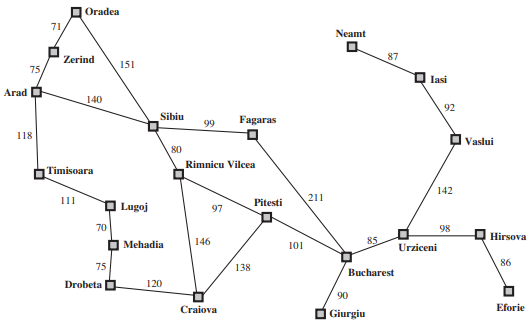
\includegraphics[width=.8\textwidth]{bulgaria2.png}
\end{figure}
City: (f(city), g(city), h(city)) \\
Lugoj: (244, 0, 244) (Starting cell, \textbf{1st cell expanded})\\
\tab Mehadia: (311, 70, 241) \textbf{2nd cell expanded} \\
\tab Timisoara: (440, 111, 329) \\
Mehadia: (311, 70, 241) \\
\tab Drobeta: (387, 145, 242) \textbf{3rd cell expanded} \\
Drobeta: (387, 145, 242) \\
\tab Craiova: (425, 265, 160) \textbf{4th cell expanded}\\
Craiova: (425, 265, 160) \\
\tab Pitesti: (503, 403, 100) \\
\tab Rimnicu Vilcea: (604, 411, 193) \\
Timisoara: (440, 111, 329) \textbf{5th cell expanded} \\
\tab Arad: (595, 229, 366) \\
Pitesti: (503, 403, 100) \textbf{6th cell expanded}\\
\tab Bucharest: (503, 503, 0) \textbf{Goal state found} \\
\newpage

\section *{Problem 2}
\begin{center}
\Tree[.1 [.2 [.4 8 
		[.9 ] ]
	   [.5 10
	         [.11 ] ] ]
	   [.3 [.6 12 
		[.13 ] ]
	   [.7 14
	         [.15 ] ] ] ]
\end{center}
(a) Assume a goal state of 11. \\
$\forall$ $S_i \in$ S, i = 0 is the first node explored. \\
Breadth first search yields S = \{1, 2, 3, 4, 5, 6, 7, 8, 9, 10, 11\} \\
Depth limitied search (L = 3) yields S = \{8, 9, 4, 10, 11\} goal state has been found at this point so no need to continue.\\
If we assume the goal state was not within depth 3 we would have S = \{8, 9, 4, 10, 11, 5, 2, 12, 13, 6, 14, 15, 7, 3, 1\} \\
Iterative Deepening Search yields \\
\tab for L = 0, S = \{1\} \\
\tab for L = 1, S = \{2, 3, 1\} \\
\tab for L = 2, S = \{4, 5, 2, 6, 7, 3, 1\} \\
\tab for L = 3, S = \{8, 9, 4, 10, 11\} \\
\tab Total searched nodes are $S_t$ = \{1, 2, 3, 1, 4, 5, 2, 6, 7, 3, 1, 8, 9, 4, 10 ,11\} \\
(b) Bidirectional search would work fairly well in this problem. In this problem we have a binary tree and as such for any goal state that we choose, all of its predecessors will be limited to 1 per depth. In this example we have the predecessors of our goal state: \\
\begin{center}
\Tree[.11 [.5 [.2 1 ] ] ]
\end{center}
Thus, the branching factor of our forward search, $b_f$ = 2 and the branching factor of our backwards search, $b_b$ = 1. \\
The expansion of the forward and backwards searches: \\
$S_f$ = \{1\} $S_b$ = \{\} \\
$S_f$ = \{1\} $S_b$ = \{11\} \\
$S_f$ = \{1, 2\} $S_b$ = \{11\} \\
$S_f$ = \{1, 2\} $S_b$ = \{11, 5\} \\
$S_f$ = \{1, 2, 3\} $S_b$ = \{11, 5\} \\
$S_f$ = \{1, 2, 3\} $S_b$ = \{11, 5, 2\} \\
There is no need to continue because a cooresponding frontier has been found and as such a path exists from the start node to goal node. \\
\newpage
\section *{Problem 3}
The phrase "search A is a special case of search B" is quite vague. I will define this phrase, A is a special case of B, as: If search A builds upon the search algorithm of search B then A is a special case of B. Otherwise B might build upon A and have similar algorithms but that does not make A a special case of B.
(a) False, breadth-first search is not a special case of uniform-cost search. However, uniform-cost search IS a special case of breadth-first search in which a priority queue is implemented. \\
(b) False\\
(c) Technically true? Uniform-cost search is simply A* search with a heuristic value, (h(n)) = 0 at all steps. Though it would be more appropriate to say that A* search is a special case of uniform-cost search.\\
(d) Depth-first graph search is not guaranteed to return an optimal solution. It is possible that multiple goal states exist and due to the nature of DFS the deepest nodes are explored first. Hence, a solution could be found first while a more shallow goal state exists in a different branch that has not yet been explored.\\
(e) If all path costs are uniform then breadth-first graph search is guaranteed to return an optimal solution. However, if path costs are not uniform a more precise algorithm is required to return an optimal solution; such as the uniform-cost search.\\
(f) Uniform-cost graph search is guaranteed to return an optimal solution. This algorithm solves the issue faced by BFS when it encounters path costs that are not uniform by implementing a priority queue.\\
(g) True\\
(h) True\\
(i) True \\




\section *{Problem 4}
Iterative deepening has the same time complexity as breadth first search, but has a space complexity more similiar to depth first search, which is non exponential in comparison to the exponential space complexity of breadth first search. \\
A disadvantage of iterative deepening is that while the time complexity of iterative deepening and breadth first search are technically both bounded by $O(b^d)$, in practice iterative deepening will in fact take marginally more time to compute because it essentially computes depth first search for every single depth. While we only really care about the final depth search, the fact remains that many iterations happened previously that did require some sort of computational power. \newpage



\section *{Problem 5}
By  the definition of a consistent heuristic: at a node n, h(n) $\leq$ c + h($n'$) where c = the cost of getting from node n to $n'$. We can think of a simple example to visualize this by imagining that the number line from 1-10 is a graph that we are examining. So our path is a straight line from 1 to 10, where all of our costs are 1. So we have for example that h(1) = 9 and h(2) = 8, the cost of getting from 1 to 2 is c = 1. So we have h(n) $\leq$ c + h($n'$) = 9 $\leq$ 1 + 8 = 9 \checkmark . In this example our heuristic is consistent and admissible. But if we were to for some reason overestimate for even a single node, our heuristic would become nonconsistent and nonadmissible. If instead of h(2) = 8, we for some reason had that h(2) = 9, our heuristic is now overestimating the cost of getting from 2 to 10 on the number line, since we know that it should only cost 8 at most. Our inequality for consistency now fails, 9 $\nleq$ 1 + 9. \\
It is now understood that for a heuristic to be consistent the heuristic must at a minimum be admissible so that the heuristic is constantly decreasing on its way to the goal.
\begin{figure}[!htb]
	\centering
	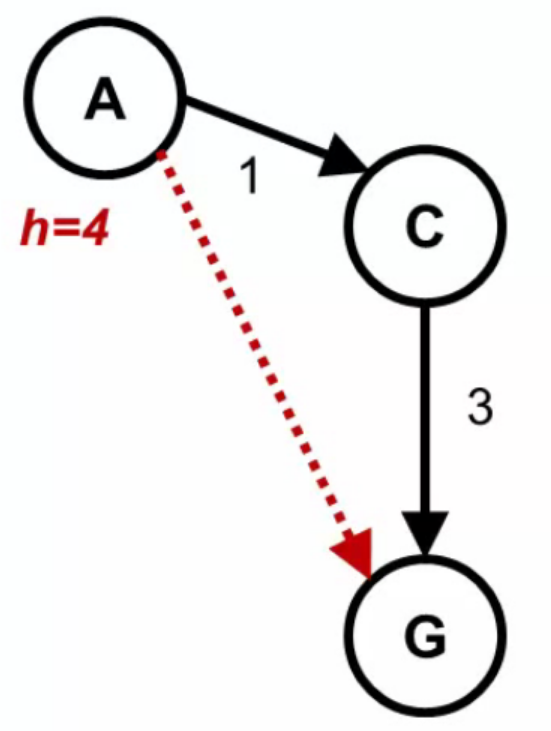
\includegraphics[width=.3\textwidth]{problem5.png}
\end{figure} \\
In this figure we have h(A) = 4, if we let h(C) = 2 then we have an admissible heuristic since h(A) $\leq$ 4 and h(C) $\leq$ 3. However, our heuristic is not consistent in this case because we have h(A) $\nleq$ c + h(C). In other words we have 4 $\nleq$ 3. So our heuristic is inconsistent, which is almost obvious since our h(A) in its computation seemingly calculated a path of cost 3 to get from node C to the goal. However our heuristic in reality produced a cost of 2 from node C to the goal node. \newpage


\section *{Problem 6}
When in a Constraint Satisfaction Problem search, it is a good heuristic to choose the variable that is most constrained first. This is because our branching factor is dependent on how many constraints are present, we would rather fail as fast as possible so as to not explore branches unnecessairily. On the other hand, we take the opposite approach with variables. We prefer to use the most flexible variables first because they are more likely to succeed, and in the off-chance that they do not succeed; all other variables must be checked anyway. So by choosing the most flexible or least constraining variable we can attempt to short circuit if it is possible, by finding the solution first.


\section *{Problem 7}
(a) The best move for the MAX player using the minimax procedure is C, because that is where the maximum minimum gain occurs. \\
(b) and (c):
\begin{figure}[!htb]
	\centering
	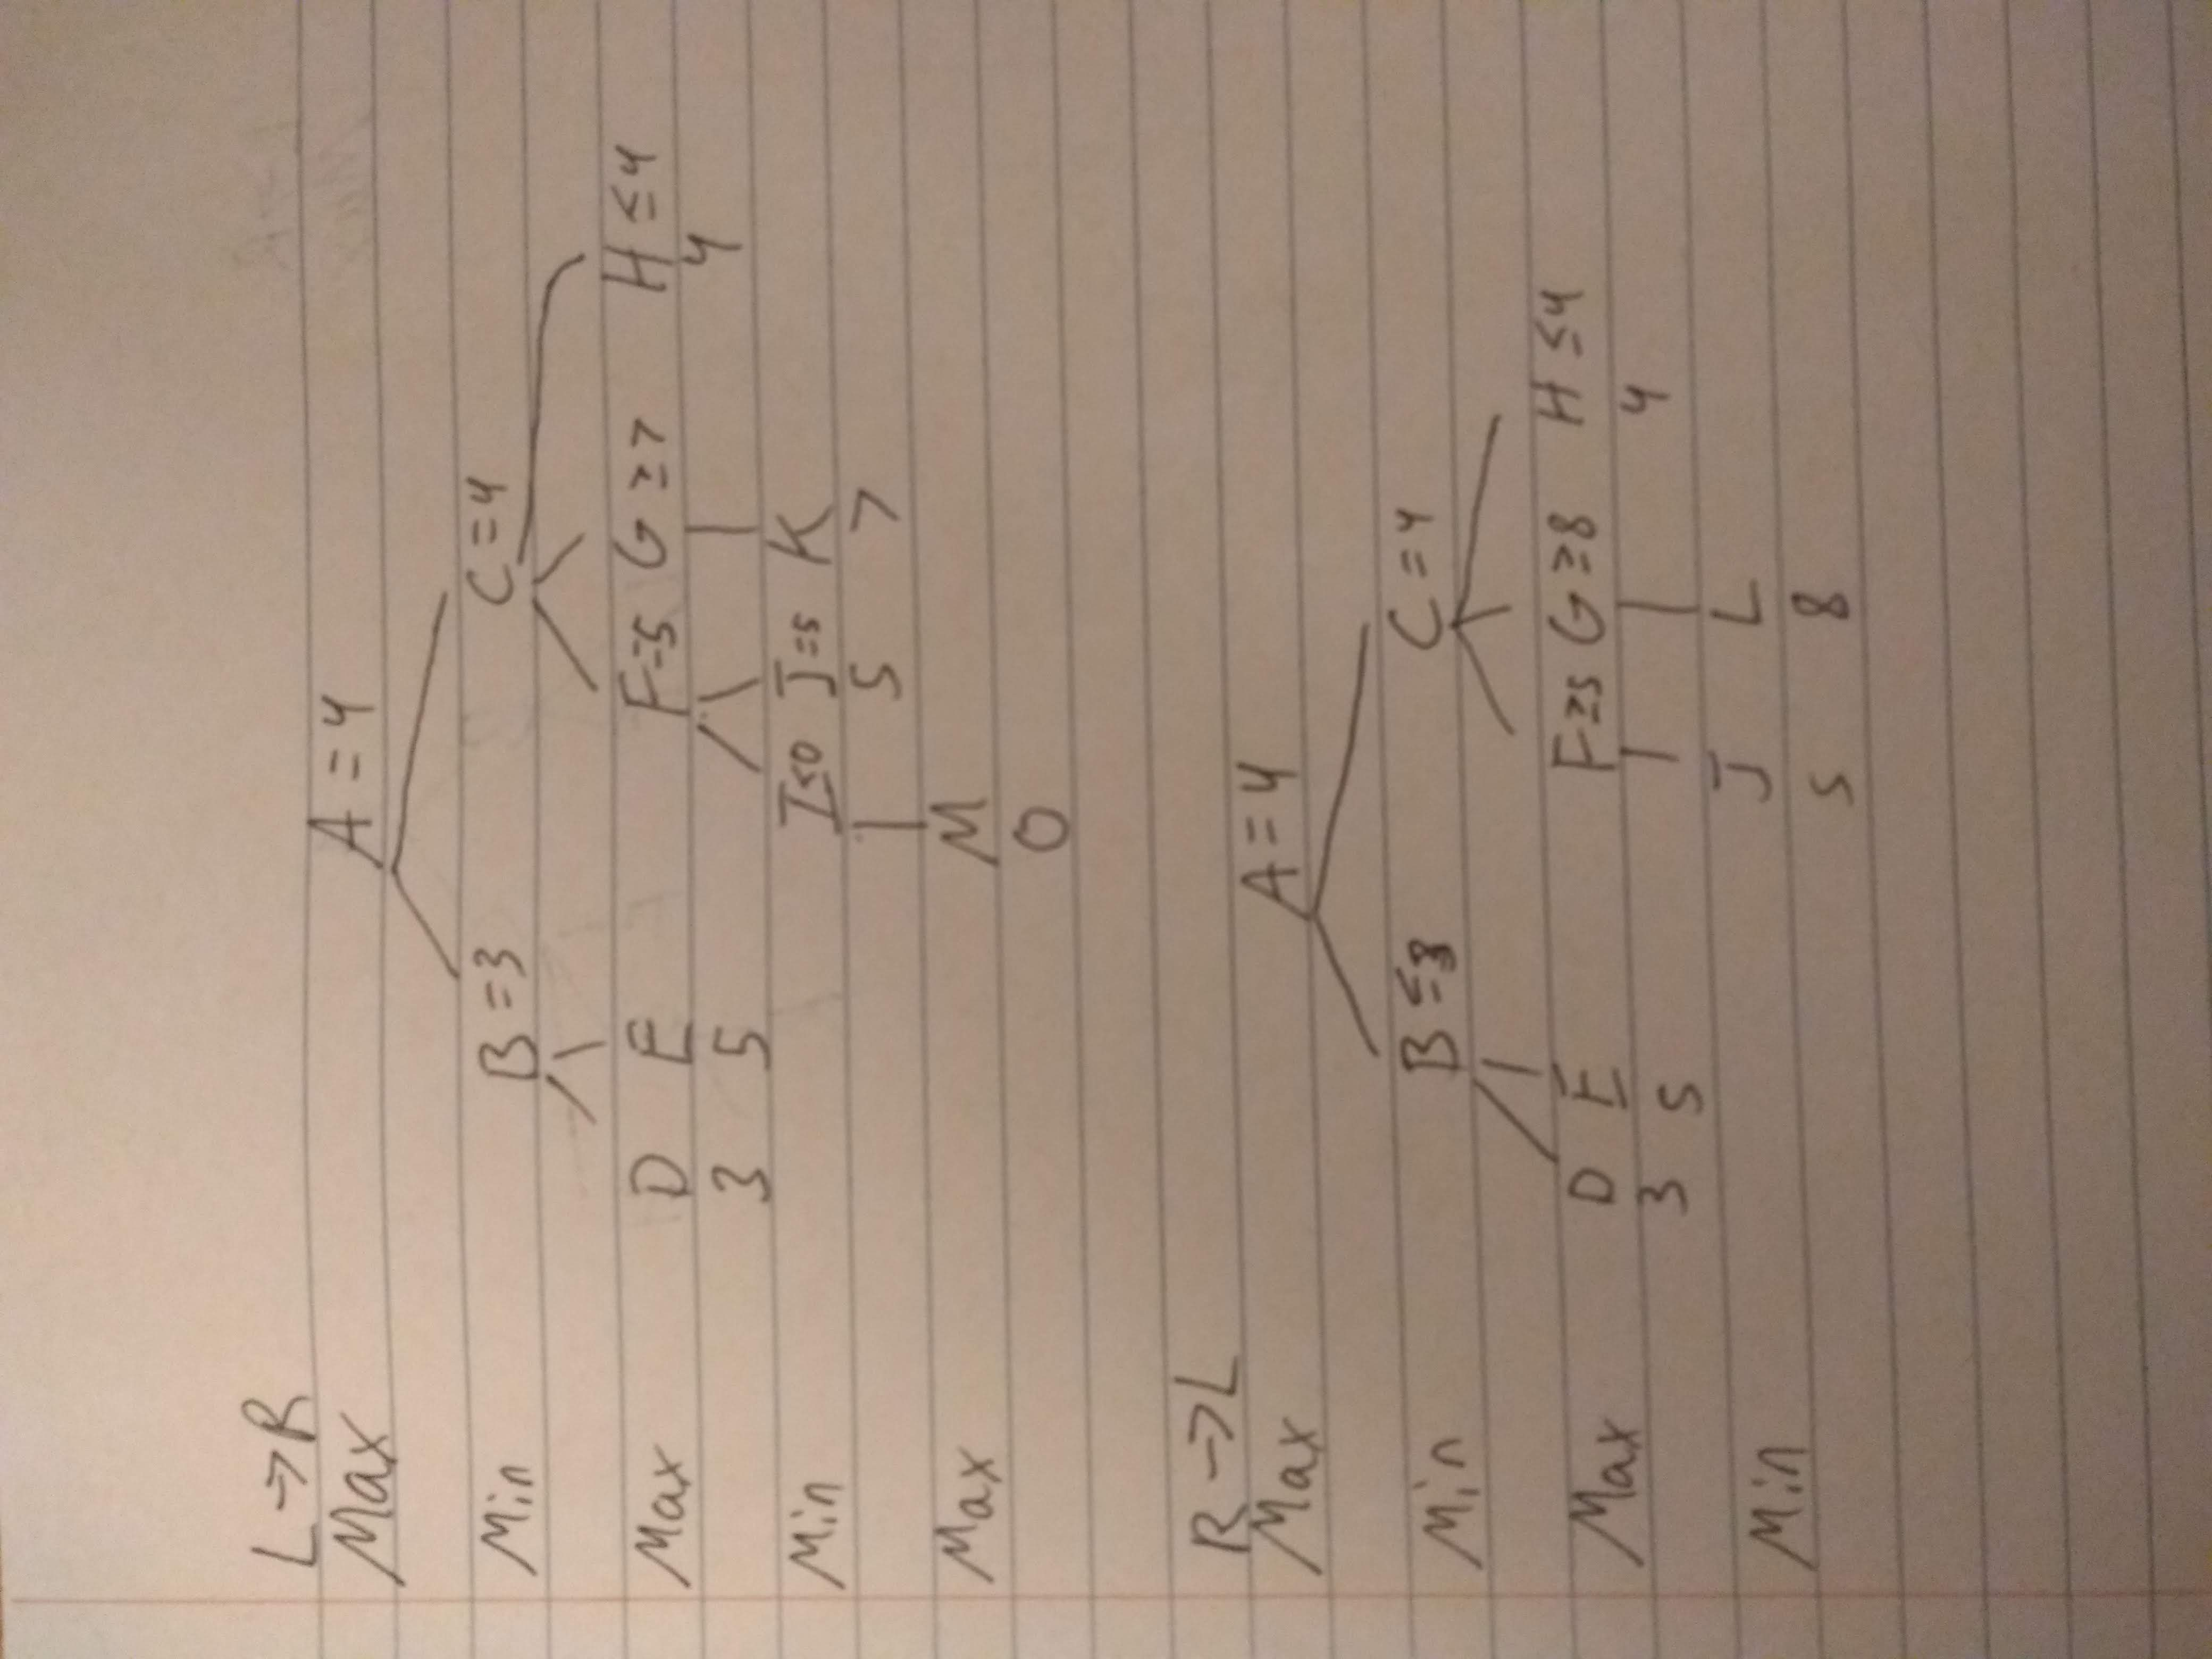
\includegraphics[width=.5\textwidth,angle=270, origin=c]{problem7.jpg}
\end{figure} 
\newpage



\section *{Problem 8}
My answers are with the assumption that both $h_1$ and $h_2$ are attempting to reach the same goal node. \\
(a) h(n) = min\{$h_1$(n),$h_2$(n)\} \\
Given that $h_1$ and $h_2$ are admissible heuristics already, neither $h_1$ nor $h_2$ will overestimate the cost of reaching the goal from n. Therefore if we take the min\{$h_1$(n), $h_2$(n)\}, we will certainly never overestimate the cost of reaching the goal from n. This is because we are essentially just choosing one of two admissible heuristic functions. \\
If $h_1$ and $h_2$ are consistent  than h is also consistent. We can use the same ideology as when $h_1$ and $h_2$ were admissible heuristics. Since, they are both consistent heuristics, we are always choosing a consistent heuristic, and the smaller of the two consistent heuristics at that. It is also highly likely that since both heuristics are consistent, h(n) will probably be consistent with picking either heuristic up until it reaches the goal.\\ \\
(b) h(n) = $\omega h_1$(n) + (1 - $\omega$)$h_2$(n), where 0 $\leq \omega \leq$ 1 \\
Again, assuming that $h_1$ and $h_2$ are admissible, then h is also admissible. Since $\omega$ can be anywhere between 0 and 1; our edge cases are therefore 0 and 1 which yields us with simply $h_2$ and $h_1$ respectively. Therefore in our edge cases, h is clearly an admissible heuristic as well. If $\omega$ is in between 0 and 1, $\omega$ + (1 - $\omega$) will always equal 1. For example if $\omega$ = 0.5: 0.5 + (1 - 0.5) = 1. Thus our factor of $h_1$ and $h_2$ is always a total of 1. If we take two things that are individually $\leq$ N and cut them both in half; when we add them together they will still be $\leq$ N because they inherently must be $\leq$ N in the first place. \\
If $h_1$ and $h_2$ are now consistent we have:\\ h(n) $\leq$ $\omega h_1(n') + (1-\omega)h_2(n')+c(n, a, n') \leq h(n') + c(n, a, n')$\\
So this consistency of h holds. \\ \\
(c) h(n) = max\{$h_1$(n),$h_2$(n)\} \\
For the same reason that (a) was admissible, (c) is also admissible when $h_1$ and $h_2$ are admissible. No matter which heuristic we pick, we are picking a heuristic that does not overestimate the goal, thus h(n) does not overestimate the goal. \\
In the cases that $h_1$ and $h_2$ are consistent h is again consistent. Since we have shown that h is admissible, the only difference is that we are adding the cost of getting from n to $n'$ in any case. For example we have h(n) $\leq$ h($n'$) + c; which is the definition of a consistent heuristic.\\ \\
If I were to use one of these heuristics for A* search algorithm I would likely choose (a) because it is, in my opinion, the heuristic that will reach the goal node with the least explored nodes. Also (a) and (c) require less computation per heuristic as compared to (b), which can be impactful with a large scale A* search.
\newpage
\section *{Problem 9}
(a) The random part of simulated annealing is not necessary in the situation that the problem at hand only contains one area in which it increases, in other words; when the problem only has one possible maximum such that the local maximum (the only maximum possible) is always equivalent to the global maximum. In this situation there is no difference between basic hill-climbing and simulated annealing because both will always reach the global maximum. \\
(b) The hill-climbing part of simulated annealing is not necessary when either the entire function is constant, or the entire function is close enough to constant that the randomness is too slow to be worth it. \\
(c) Simulated annealing is useful in the situation that the cost function is well structured and has at least a few, but preferably many local maxima such that hill climbing is likely has no hope of finding the global maximum unless by pure luck. A good visual example of a well structured cost function is something like this, or even more complex. \\
\begin{figure}[!htb]
	\centering
	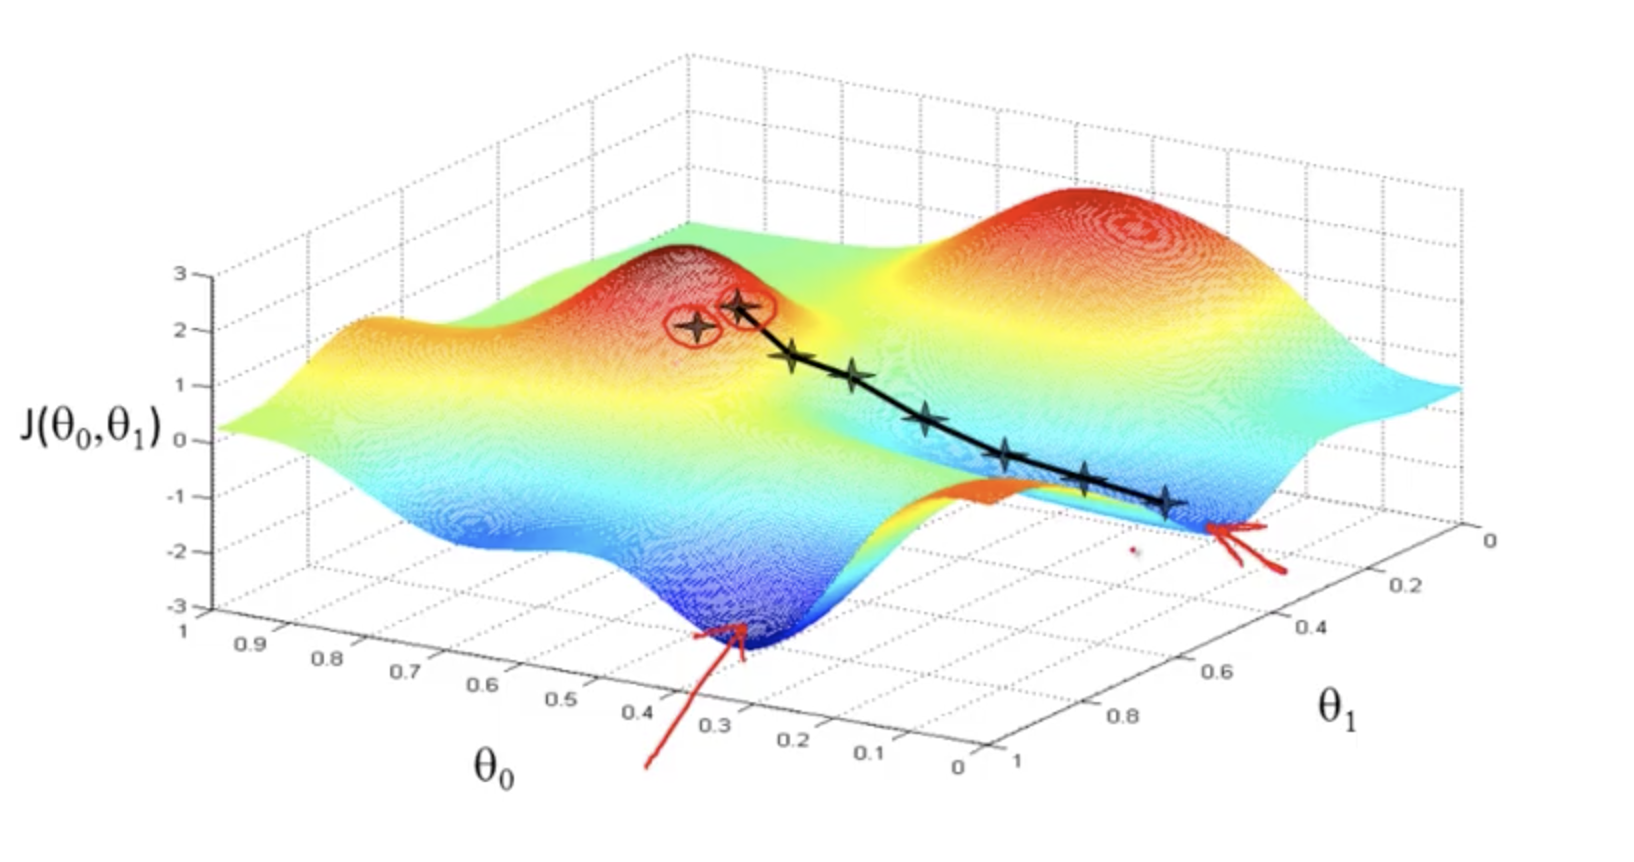
\includegraphics[width=.8\textwidth]{costfunction.png}
\end{figure} \\
(d) Given that we know the value of each state we visit and since we only choose our next state if it is an increase from our current state; instead of reducing the randomness of our hops at a consistent rate, it would perhaps be beneficial to increase or decrease the hops at a rate relative to the amount of increase we are seeing. For example, if we were evaluating only very minor improvements in our search for the global maximum, we could adjust our hops to be exploring further from our current location to get to the global maximum first. Some caution would have to be taken as to ensure the relative distance increase does not accidentally hop over the global maximum and result in no solution. \\
(e) If we had enough memory to hold two million states with simulated annealing we could adjust the algorithm to help us understand when our algorithm is having difficulty traversing through local optima. By storing all states we have visited previously we could implement a system such that, given a marginal increase over n states, we adjust the "shaking" or hopping that we are doing from state to state. Thus increasing the speed at which the simulated annealing algorithm conquers local optima, since the majority of time spent is likely overcoming local optima. \\
(f) To avoid the trap of local maximums with gradient ascent, you would use an improvised version called stochastic gradient ascent. Stochastic gradient ascent implements a randomness similar to simulated annealing such that the learning rate in gradient ascent is altered instead of being kept at a constant rate. As said previously though, this type of randomness influences the efficiency at the cost of optimality and can still yield a local maxima result.

\section *{Problem 10}
\begin{figure}[!htb]
	\centering
	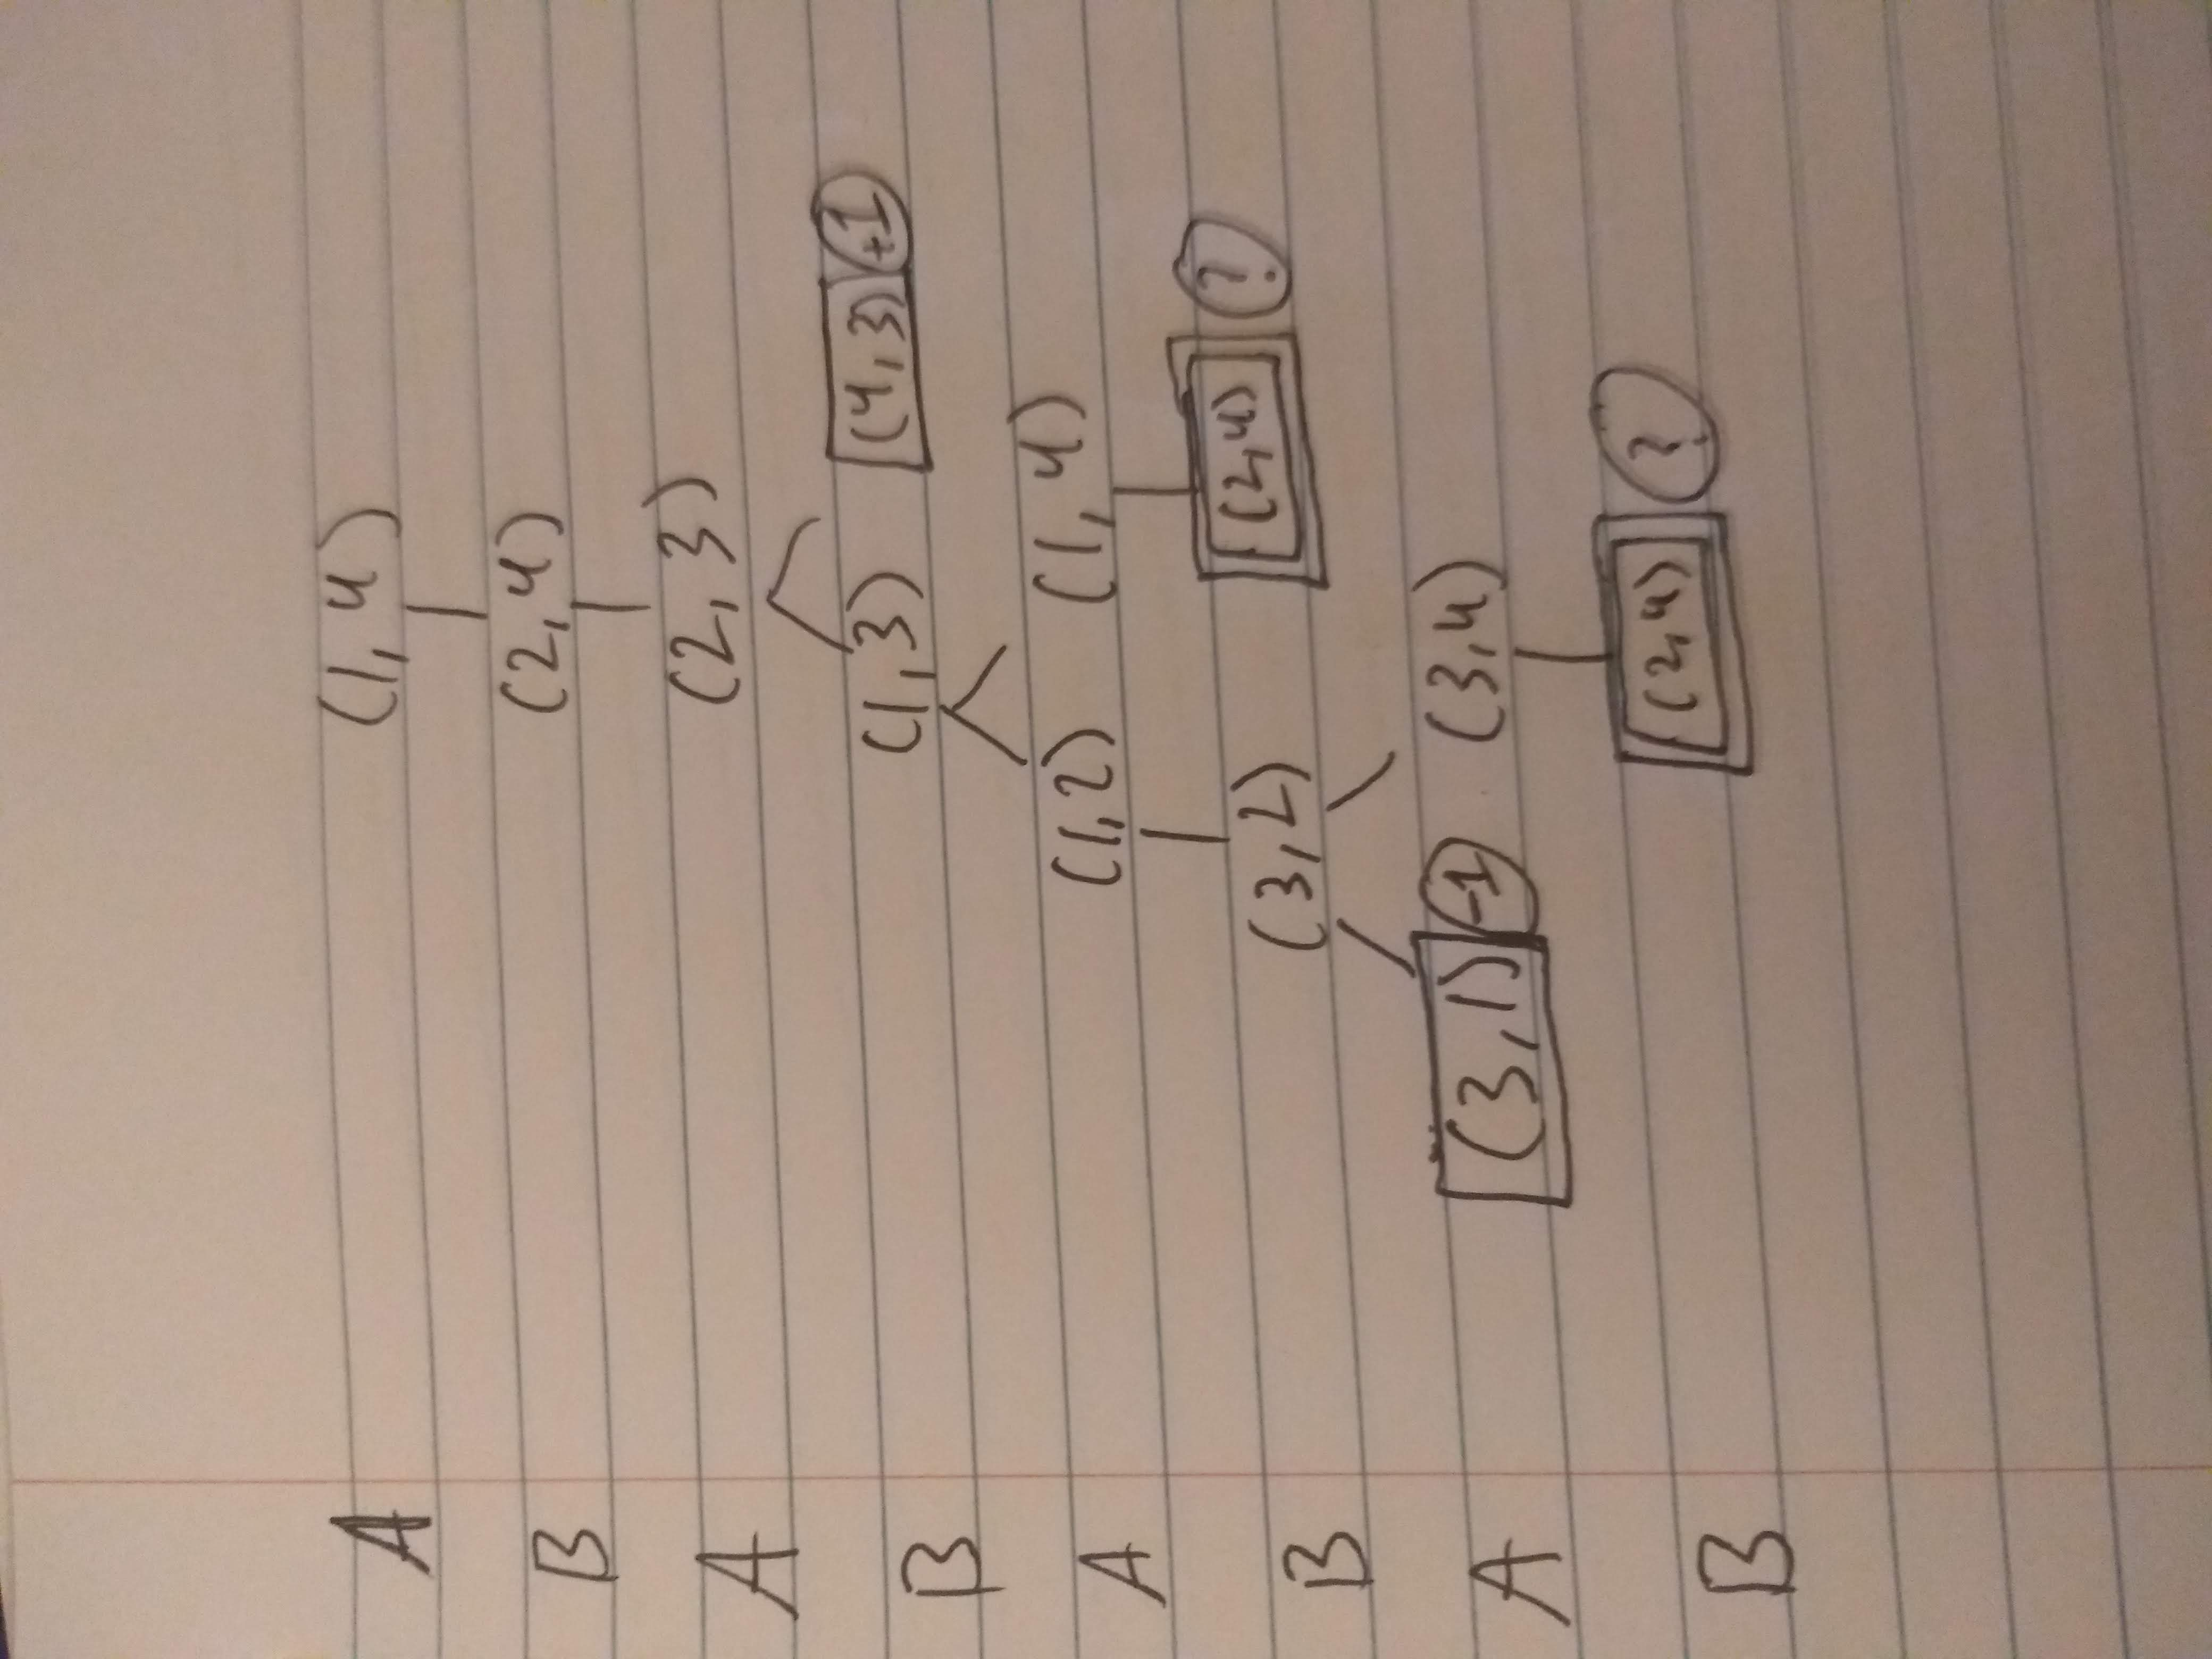
\includegraphics[width=.5\textwidth,angle=270, origin=c]{problem10.jpg}
\end{figure} 
In this game tree our only loop states that occur are (2, 4). We also take note that at every occurence of (2,4) the player that must choose their move next is player B. Thus (2, 4) always leads to (2, 3). Now that it is player A's turn, an optimal player will always win since the player's two options are either to win outright or to move back to state 1. This game is simple enough and so heavily favored towards player A to win that player A should always win. Thus, we can regard the ? values as +1 since player A should definitely choose to win and is always given the opportunity to win.



\end{document}